\documentclass[border=1mm]{standalone}
\usepackage{tikz,tkz-euclide}
\usepackage{pgfplots}
\usetikzlibrary{arrows,calc,patterns,intersections}
\begin{document}


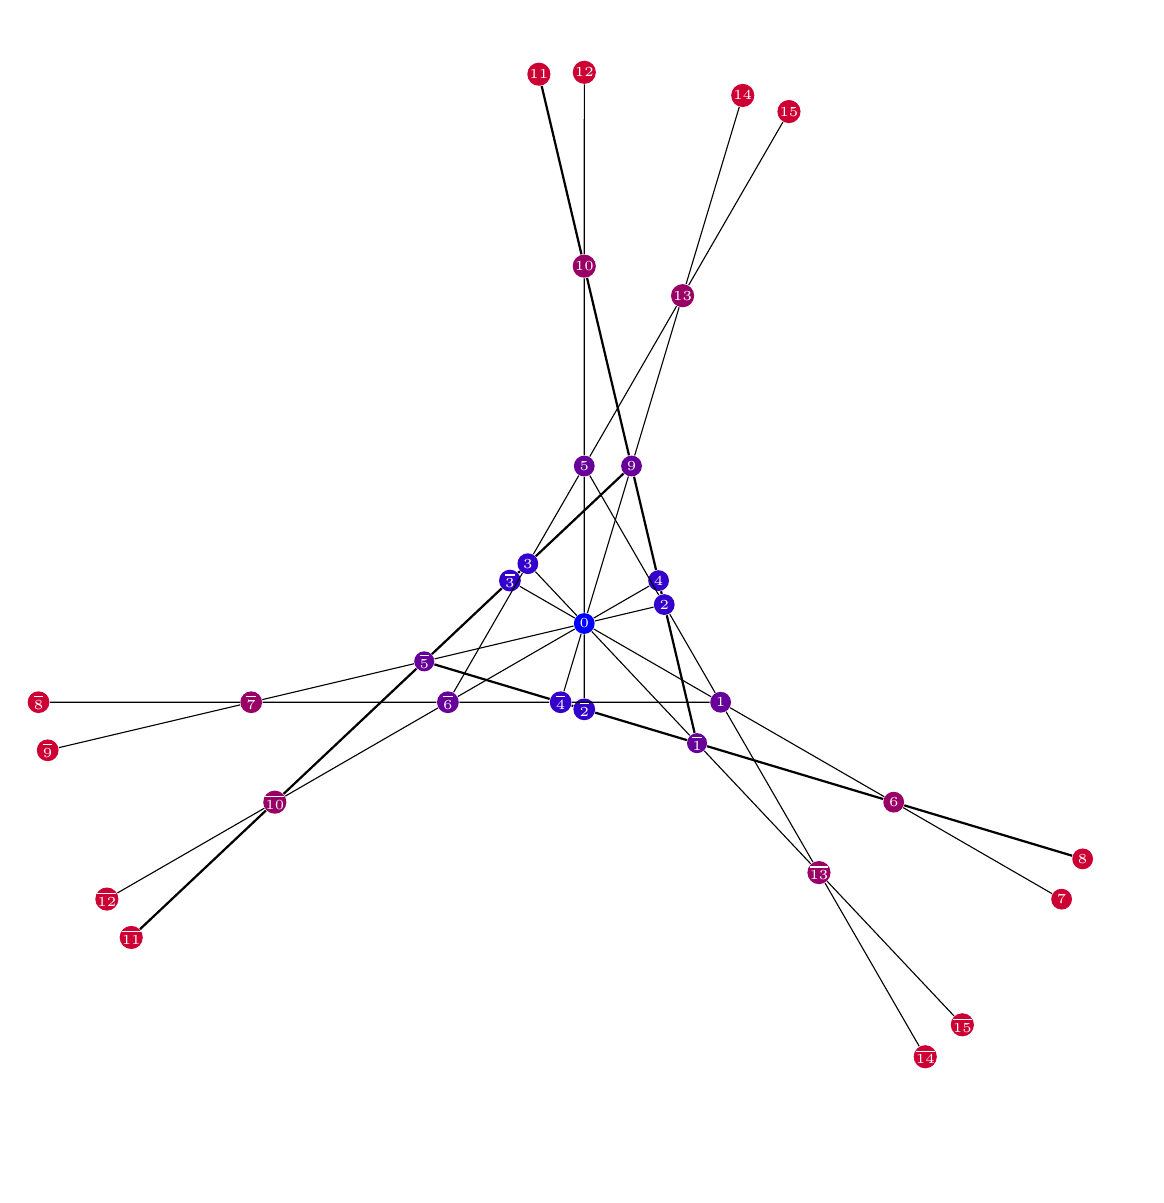
\begin{tikzpicture}[scale=2]

\tikzset{
    dot/.style={circle,inner sep=1pt,fill,label={\tiny #1},name=#1}}

\node[dot, fill=blue!100!red] (z) at (0,0) {\tiny \textcolor{white}{$0$}};
\coordinate (h) at (0,1);

\node[dot, fill=blue!60!red] (p9) at (0.3,1) {\tiny \textcolor{white}{$9$}};

\node[dot, fill=blue!60!red] (m5) at ($(0,0)!1!120:(p9)$) {\tiny \textcolor{white}{\!\!$\overline 5$\!\!}};

\node[dot, fill=blue!60!red] (m1) at ($(0,0)!1!240:(p9)$) {\tiny \textcolor{white}{\!\!$\overline 1$\!\!}};

\coordinate (i4) at (intersection of z--p9 and m5--m1);
\node[dot, fill=blue!80!red] (m4) at (i4) {\tiny \textcolor{white}{\!$\overline 4$\!}};
\node[dot, fill=blue!80!red] (p2) at ($(0,0)!1!120:(i4)$) {\tiny \textcolor{white}{$2$}};
\node[dot, fill=blue!80!red] (p3) at ($(0,0)!1!240:(i4)$) {\tiny \textcolor{white}{$3$}};

\coordinate (i2) at (intersection of z--h and m5--m1);
\node[dot, fill=blue!80!red] (m2) at (i2) {\tiny \textcolor{white}{\!$\overline 2$\!}};
\node[dot, fill=blue!80!red] (p4) at ($(0,0)!1!120:(i2)$) {\tiny \textcolor{white}{$4$}};
\node[dot, fill=blue!80!red] (m3) at ($(0,0)!1!240:(i2)$) {\tiny \textcolor{white}{\!$\overline 3$\!}};

\coordinate (p3x) at ($(p3) + (60:1)$);
\coordinate (m4x) at ($(m4) + (180:1)$);

\coordinate (i5) at (intersection of p3--p3x and m4--m4x);
\node[dot, fill=blue!60!red] (m6) at (i5) {\tiny \textcolor{white}{\!$\overline 6$\!}};
\node[dot, fill=blue!60!red] (p1) at ($(0,0)!1!120:(i5)$) {\tiny \textcolor{white}{$1$}};
\node[dot, fill=blue!60!red] (p5) at ($(0,0)!1!240:(i5)$) {\tiny \textcolor{white}{$5$}};

\coordinate (i7) at (intersection of m2--p5 and m1--p9);
\node[dot, fill=blue!40!red] (p10) at (i7) {\tiny \textcolor{white}{\!$10$\!}};
\node[dot, fill=blue!40!red] (m10) at ($(0,0)!1!120:(i7)$) {\tiny \textcolor{white}{\!\!$\overline {10}$\!\!}};
\node[dot, fill=blue!40!red] (p6) at ($(0,0)!1!240:(i7)$) {\tiny \textcolor{white}{${6}$}};

\coordinate (i9) at (intersection of m6--p5 and m4--p9);
\node[dot, fill=blue!40!red] (p13) at (i9) {\tiny \textcolor{white}{\!$13$\!}};
\node[dot, fill=blue!40!red] (m7) at ($(0,0)!1!120:(i9)$) {\tiny \textcolor{white}{\!$\overline 7$\!}};
\node[dot, fill=blue!40!red] (m13) at ($(0,0)!1!240:(i9)$) {\tiny \textcolor{white}{\!\!$\overline{13}$\!\!}};

\path[name path=circle] (0,0) circle (3.5);

\path[name path=l1] (m2) -- ($(m2)!1.5!(p10)$);
\path[name intersections={of=l1 and circle, by=i8}];
\node[dot, fill=blue!20!red] (p12) at (i8) {\tiny \textcolor{white}{\!${12}$\!}};
\node[dot, fill=blue!20!red] (m12) at ($(0,0)!1!120:(i8)$) {\tiny \textcolor{white}{\!\!$\overline{12}$\!\!}};
\node[dot, fill=blue!20!red] (p7) at ($(0,0)!1!240:(i8)$) {\tiny \textcolor{white}{${7}$}};

\path[name path=l2] (m1) -- ($(m1)!1.5!(p10)$);
\path[name intersections={of=l2 and circle, by=i10}];
\node[dot, fill=blue!20!red] (p11) at (i10) {\tiny \textcolor{white}{\!${11}$\!}};
\node[dot, fill=blue!20!red] (m11) at ($(0,0)!1!120:(i10)$) {\tiny \textcolor{white}{\!\!$\overline{11}$\!\!}};
\node[dot, fill=blue!20!red] (p8) at ($(0,0)!1!240:(i10)$) {\tiny \textcolor{white}{${8}$}};

\path[name path=l3] (m4) -- ($(m4)!1.5!(p13)$);
\path[name intersections={of=l3 and circle, by=i12}];
\node[dot, fill=blue!20!red] (p14) at (i12) {\tiny \textcolor{white}{\!${14}$\!}};
\node[dot, fill=blue!20!red] (m9) at ($(0,0)!1!120:(i12)$) {\tiny \textcolor{white}{\!$\overline{9}$\!}};
\node[dot, fill=blue!20!red] (m15) at ($(0,0)!1!240:(i12)$) {\tiny \textcolor{white}{\!\!$\overline{15}$\!\!}};

\path[name path=l4] (m6) -- ($(m6)!1.5!(p13)$);
\path[name intersections={of=l4 and circle, by=i14}];
\node[dot, fill=blue!20!red] (p15) at (i14) {\tiny \textcolor{white}{\!${15}$\!}};
\node[dot, fill=blue!20!red] (m8) at ($(0,0)!1!120:(i14)$) {\tiny \textcolor{white}{\!$\overline{8}$\!}};
\node[dot, fill=blue!20!red] (m14) at ($(0,0)!1!240:(i14)$) {\tiny \textcolor{white}{\!\!$\overline{14}$\!\!}};

\draw[thick] (m5) -- (m4) -- (m2) -- (m1) -- (p6) -- (p8);
\draw[thick] (m1) -- (p2) -- (p4) -- (p9) -- (p10) -- (p11);
\draw[thick] (p9) -- (p3) -- (m3) -- (m5) -- (m10) -- (m11);

\draw (m3) -- (z) -- (p1) -- (p6) -- (p7);
\draw (m2) -- (z) -- (p5) -- (p10) -- (p12);
\draw (m4) -- (z) -- (p9) -- (p13) -- (p14);

\draw (p2) -- (z) -- (m5) -- (m7) -- (m9);
\draw (p3) -- (z) -- (m1) -- (m13) -- (m15);
\draw (p4) -- (z) -- (m6) -- (m10) -- (m12) ;

\draw (p1) -- (m4) -- (m6) -- (m7) -- (m8);
\draw (m6) -- (p3) -- (p5) -- (p13) -- (p15);
\draw (p5) -- (p2) -- (p1) -- (m13) -- (m14);


\end{tikzpicture}

\end{document}
